\documentclass{article}
\title{ROS Forklift simulation manual}
\author{Konrád Soma Kiss \and Kristóf Kukk}
\date{}
\usepackage{color}
\usepackage{graphicx}
\graphicspath{ {./images/} }

\begin{document}
\maketitle

\pagebreak

\tableofcontents

\pagebreak

\section{Main Menu}
\begin{center}
    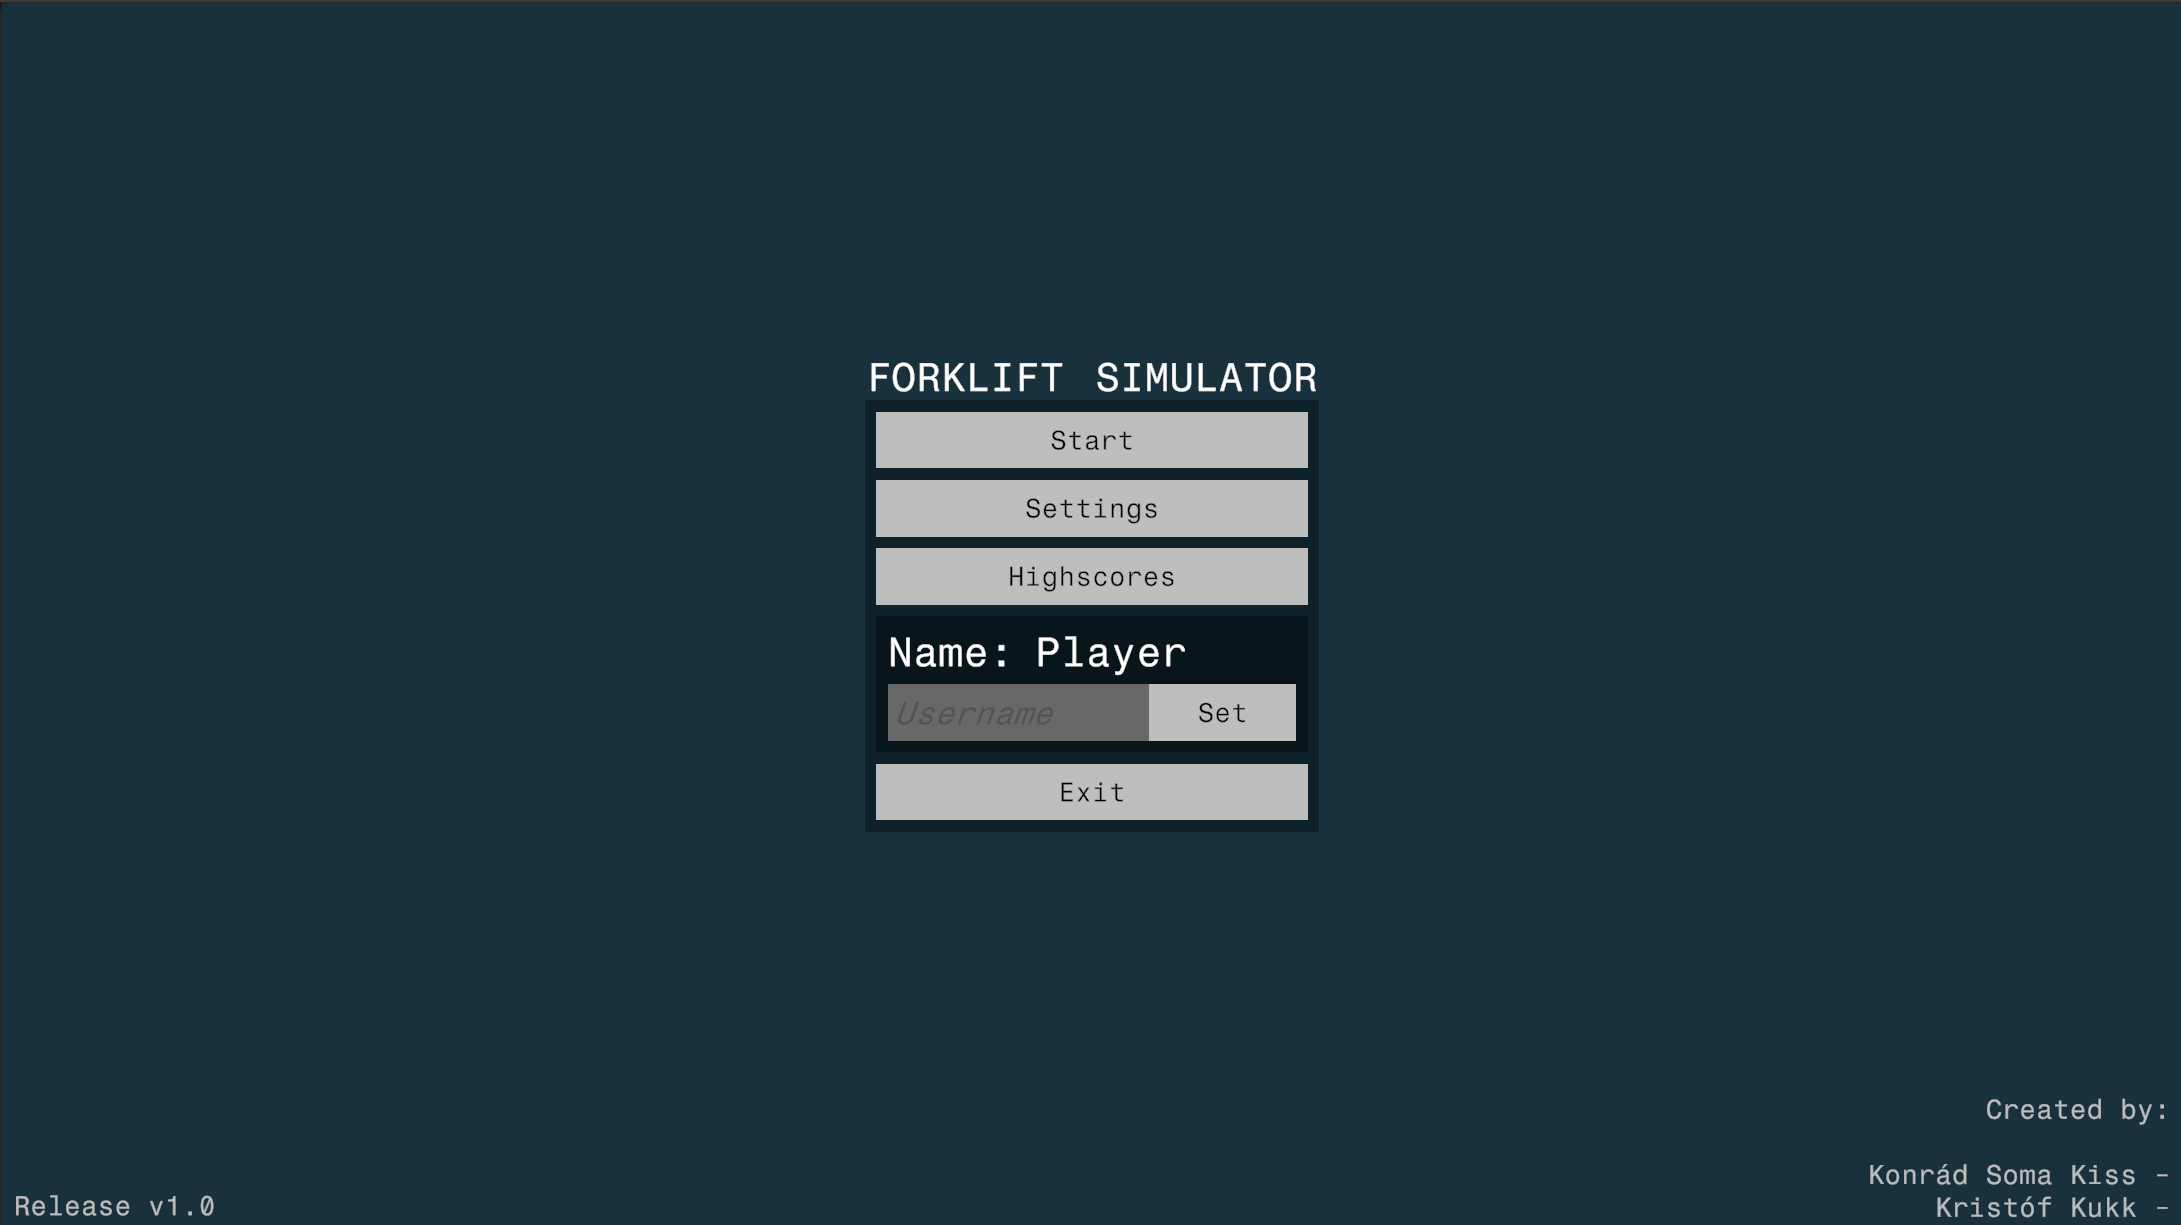
\includegraphics[width=12.1cm]{main_menu}\linebreak
    \small Screenshot of the main menu.
\end{center}

\normalsize
Most of the menu elements are self-explanatory, except the "Name" part in the middle.
That's where you can set the username, which will be used to store the achieved score.
All the scores are stored locally on the running computer.

\pagebreak

\section{Settings Menu}
\begin{center}
    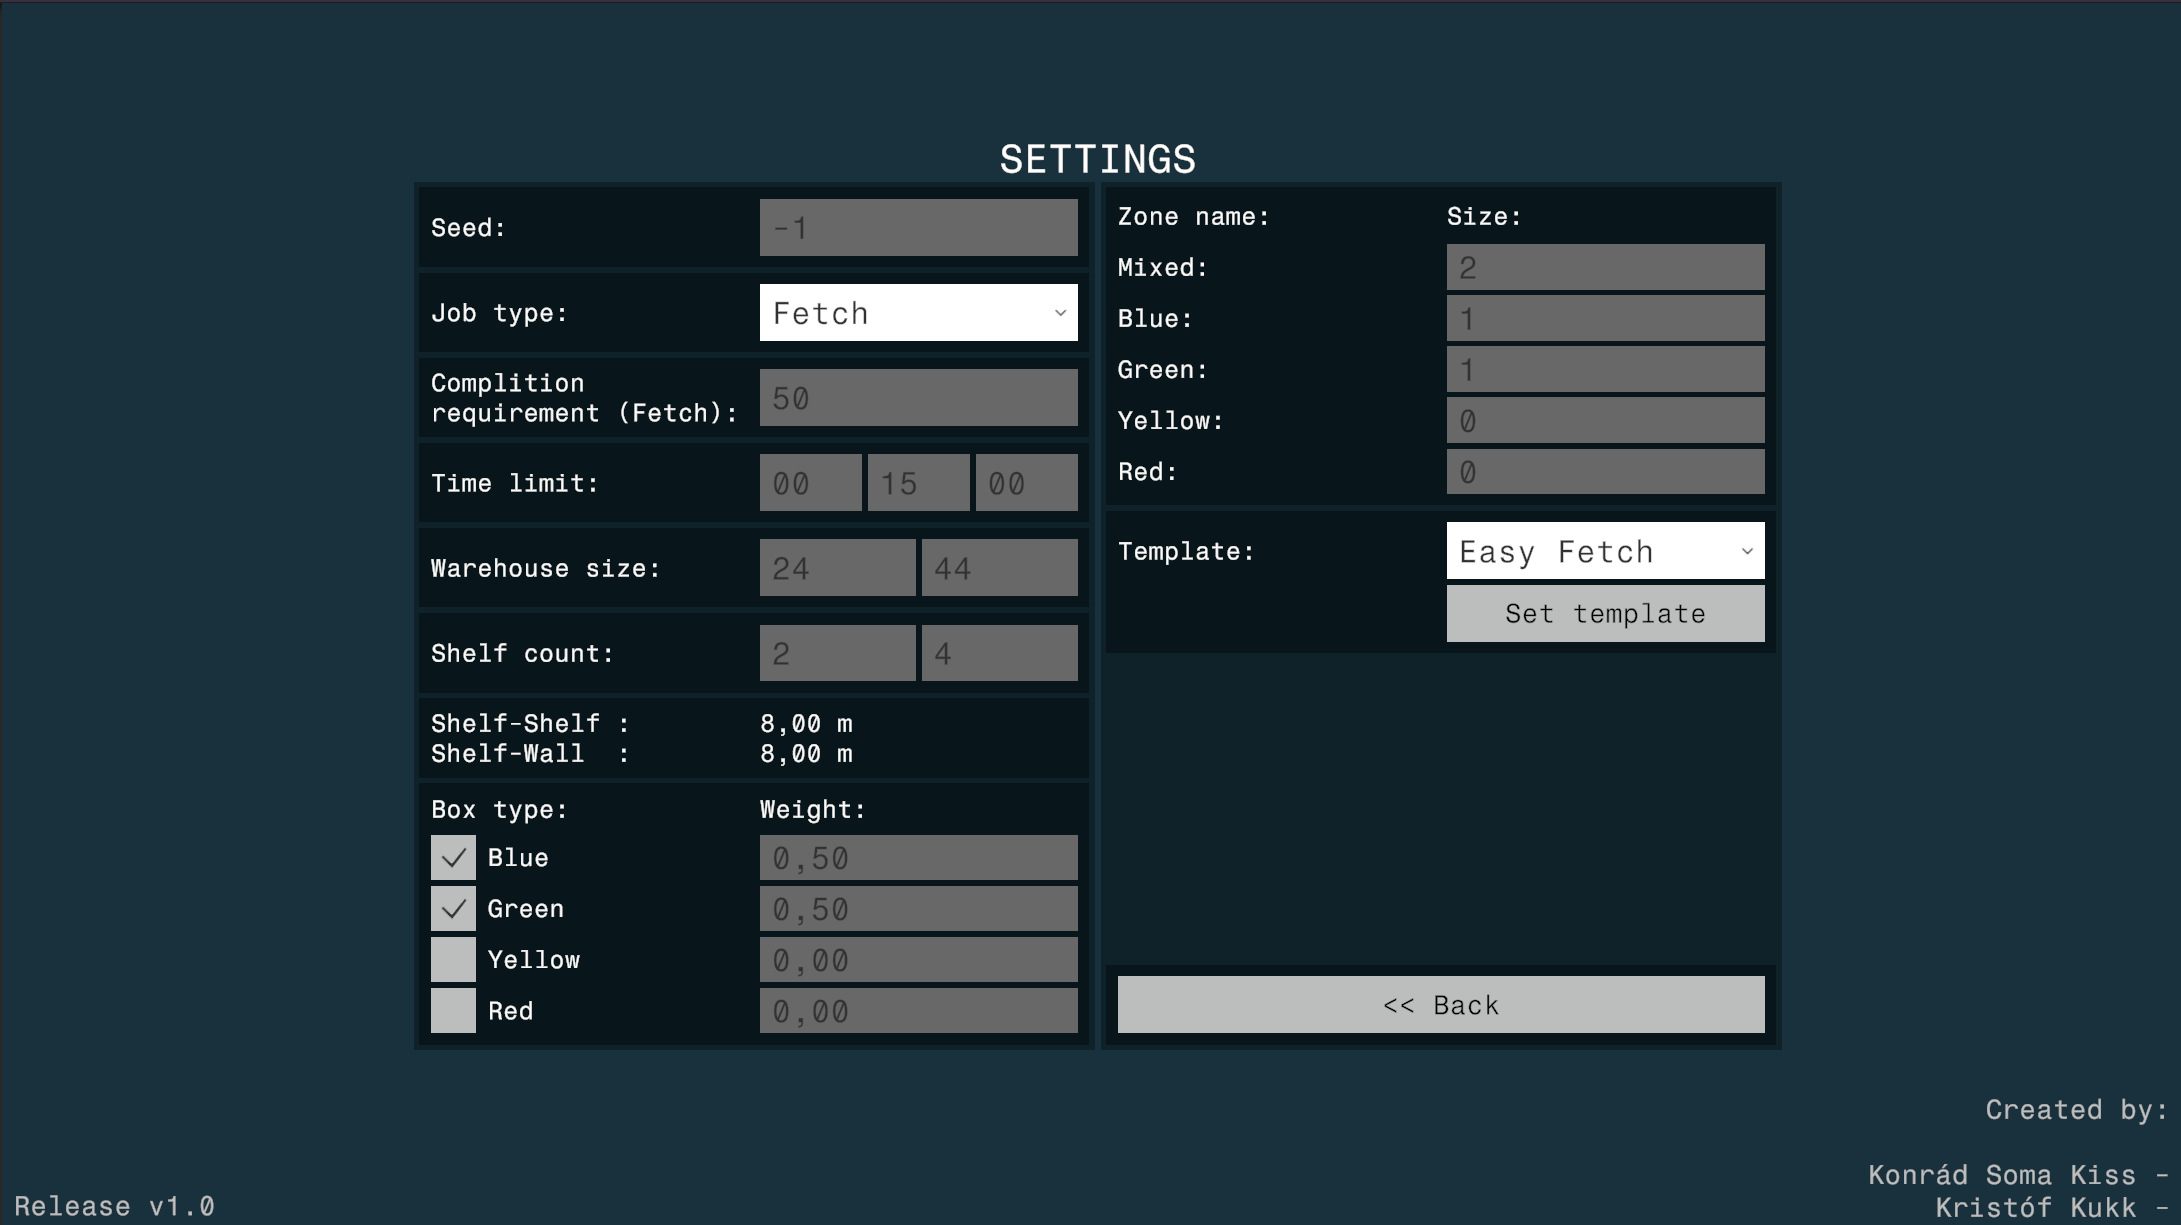
\includegraphics[width=12.1cm]{settings_menu}\linebreak
    \small Screenshot of the settings menu.
\end{center}

\normalsize
There are a lot of settings that are dependent on each other. The complete list of settings and their dependencies are as follows:
\begin{itemize}
    \item Seed - The seed used to generate everything in the level. Has no dependencies.
    \item Job type - They are as follows: 
    \begin{itemize}
        \item Fetch - A certain number of boxes will be prompted on the top right
        of the screen, and the player has to put them in the mixed (white)
        zones. Dependent on:
        \begin{itemize}
            \item Completion requirement - The amount in percentages (\%) required to complete the level. Affects the difficulty multiplier.
            \item Zone sizes - The fetchable boxes have to be able to fit within the
            mixed zones, and this behavior must be set by using the correct
            zone sizes.
        \end{itemize}
        \item Sort - All the available boxes on the mixed shelves will be prompted
        on the top right of the screen, and the player has to put them in their
        respective zones. (By color.) Dependent on:
        \begin{itemize}
            \item Completion requirement - Does not affect the amount of boxes
            required, so it defaults to 100.
            \item Zone sizes - The mixed amount of boxes must be able to fit
            within their respective zones and this behavior must be set by
            using correct zone sizes.
        \end{itemize}
    \end{itemize}
    \item Completion requirement - Only used in fetch mode. The required (\%) amount of boxes
    to complete the level. Has no dependencies.
    \item Time limit - Pretty self-explanatory, sets the time limit at which the level ends.
    Affects the difficulty multiplier, but it has no dependencies.
    \item Warehouse size - Sets the size of the warehouse in meters. The size on both axes must
    be a multiple of four to generate properly. Has no dependencies.
    \item Shelf count - Sets the number of shelves in the warehouse. The first number sets how many
    shelves are there in a row, and the second one sets the number of rows. The rows are 
    the number of empty zones available, which will be split up by the zone size setting. It has no
    dependencies.
    \item Shelf distances - A shown info about the Shelf-Shelf distances and the Shelf-Wall distances
    used. The distances are used to check if your other settings are set up correctly.
    If one of the values is less than the size of the forklift, or in an even worse case they're 
    less than zero, then the warehouse will be incorrectly generated. It is recommended to keep both
    values at around 8 meters. Its dependencies are:
    \begin{itemize}
        \item Warehouse size
        \item Shelf count
    \end{itemize}
    \item Box types - The different box types that are being generated can be set from here. The toggle
    in front sets whether or not to generate said box, and the amount after it sets how likely it will be
    to generate, where 1.0 means it will always generate when it has the chance to, and 0.0 means it won't
    spawn at all. It's dependent on:
    \begin{itemize}
        \item Zone sizes - The boxes require a zone in fetch mode to be generated, while they also require
        their zones in sort mode to have a valid place to fit them in.
    \end{itemize}
    \item Zone sizes - The different zones take up rows within the generated shelves. The sum of the zone
    sizes has to be equal to the number of rows (Shelf count 2nd setting). Also be aware of the fact, that
    when using fetch mode, the fetched boxes have to fit within the mixed zone, and in sort mode, all the
    boxes need to have enough space to be sorted out. It's dependent on:
    \begin{itemize}
        \item Box types - Don't generate zones, that are disabled within these settings, because they'll be
        pointless.
    \end{itemize}
\end{itemize}

\pagebreak

\section{Start Menu}
\begin{center}
    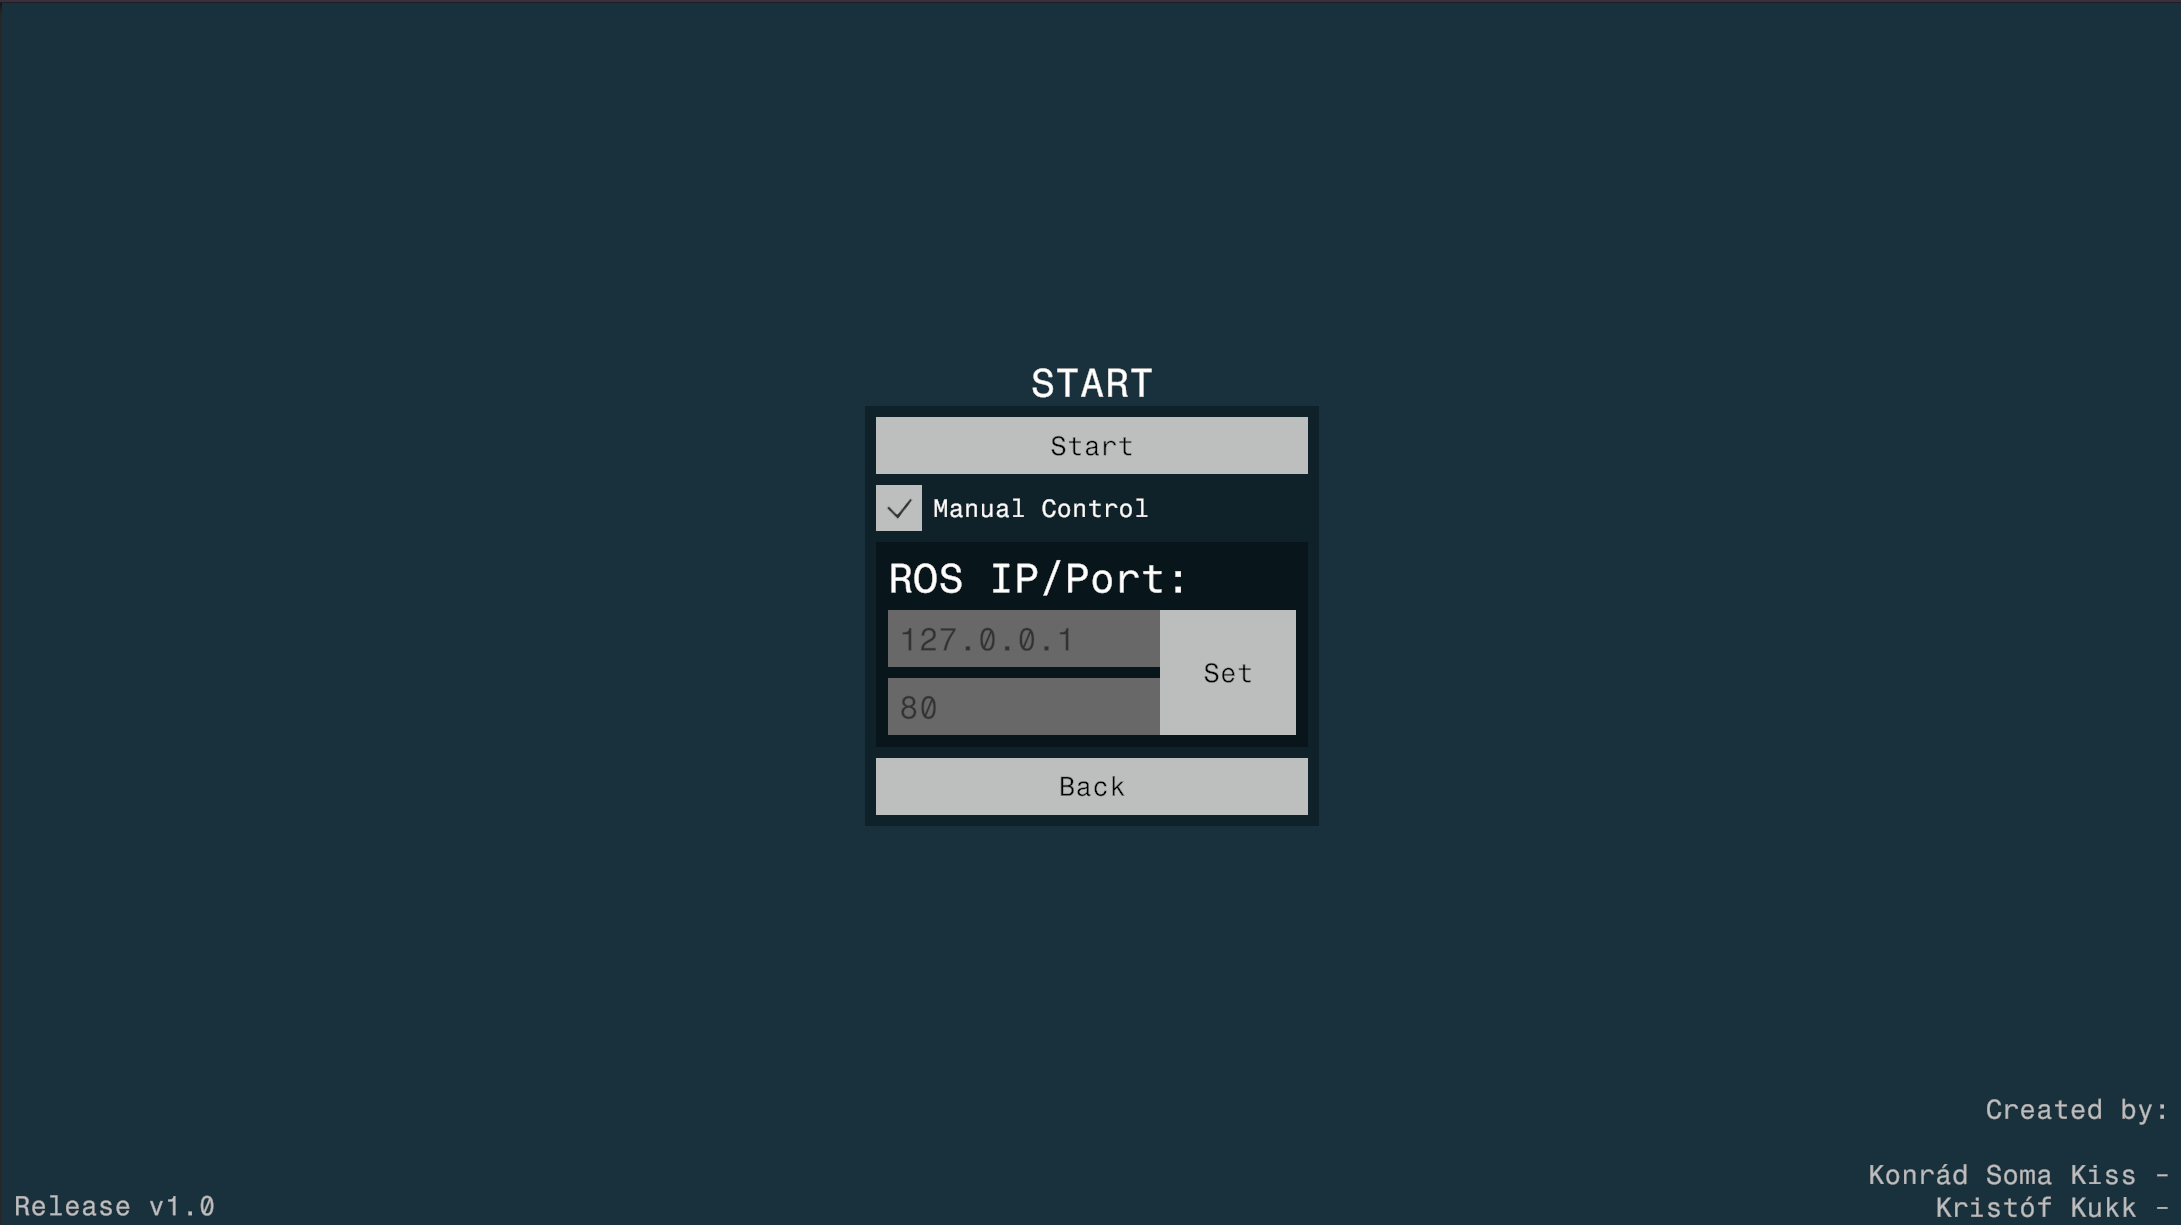
\includegraphics[width=12.1cm]{start_menu}\linebreak
    \small Screenshot of the start menu.
\end{center}

\normalsize
The start menu does not have many functionalities, but they're as follows:
\begin{itemize}
    \item Manual Control - Whether you want to use regular WASD controls to control the
    forklift or the ROS connections.
    \item ROS IP/Port - The address at which the program can access the ROS server if
    the forklift is chosen to be controlled with that.
\end{itemize}

\section{Manual Controls}
The manual controls are as follows:
\begin{itemize}
    \item W/S - Controls the main motor speed to move forwards/backward.
    \item A/D - Controls the rotation that is achieved by using the motors on the two
    sides at different rpm.
    \item Q/E - Controls the fork's motor to be lifted or lowered.
    \item ESC - Goes back to the main menu.
    \item C - Switches the locked camera to a third person freely rotating camera, and back.
\end{itemize}

\pagebreak

\section{Game Screen}
\begin{center}
    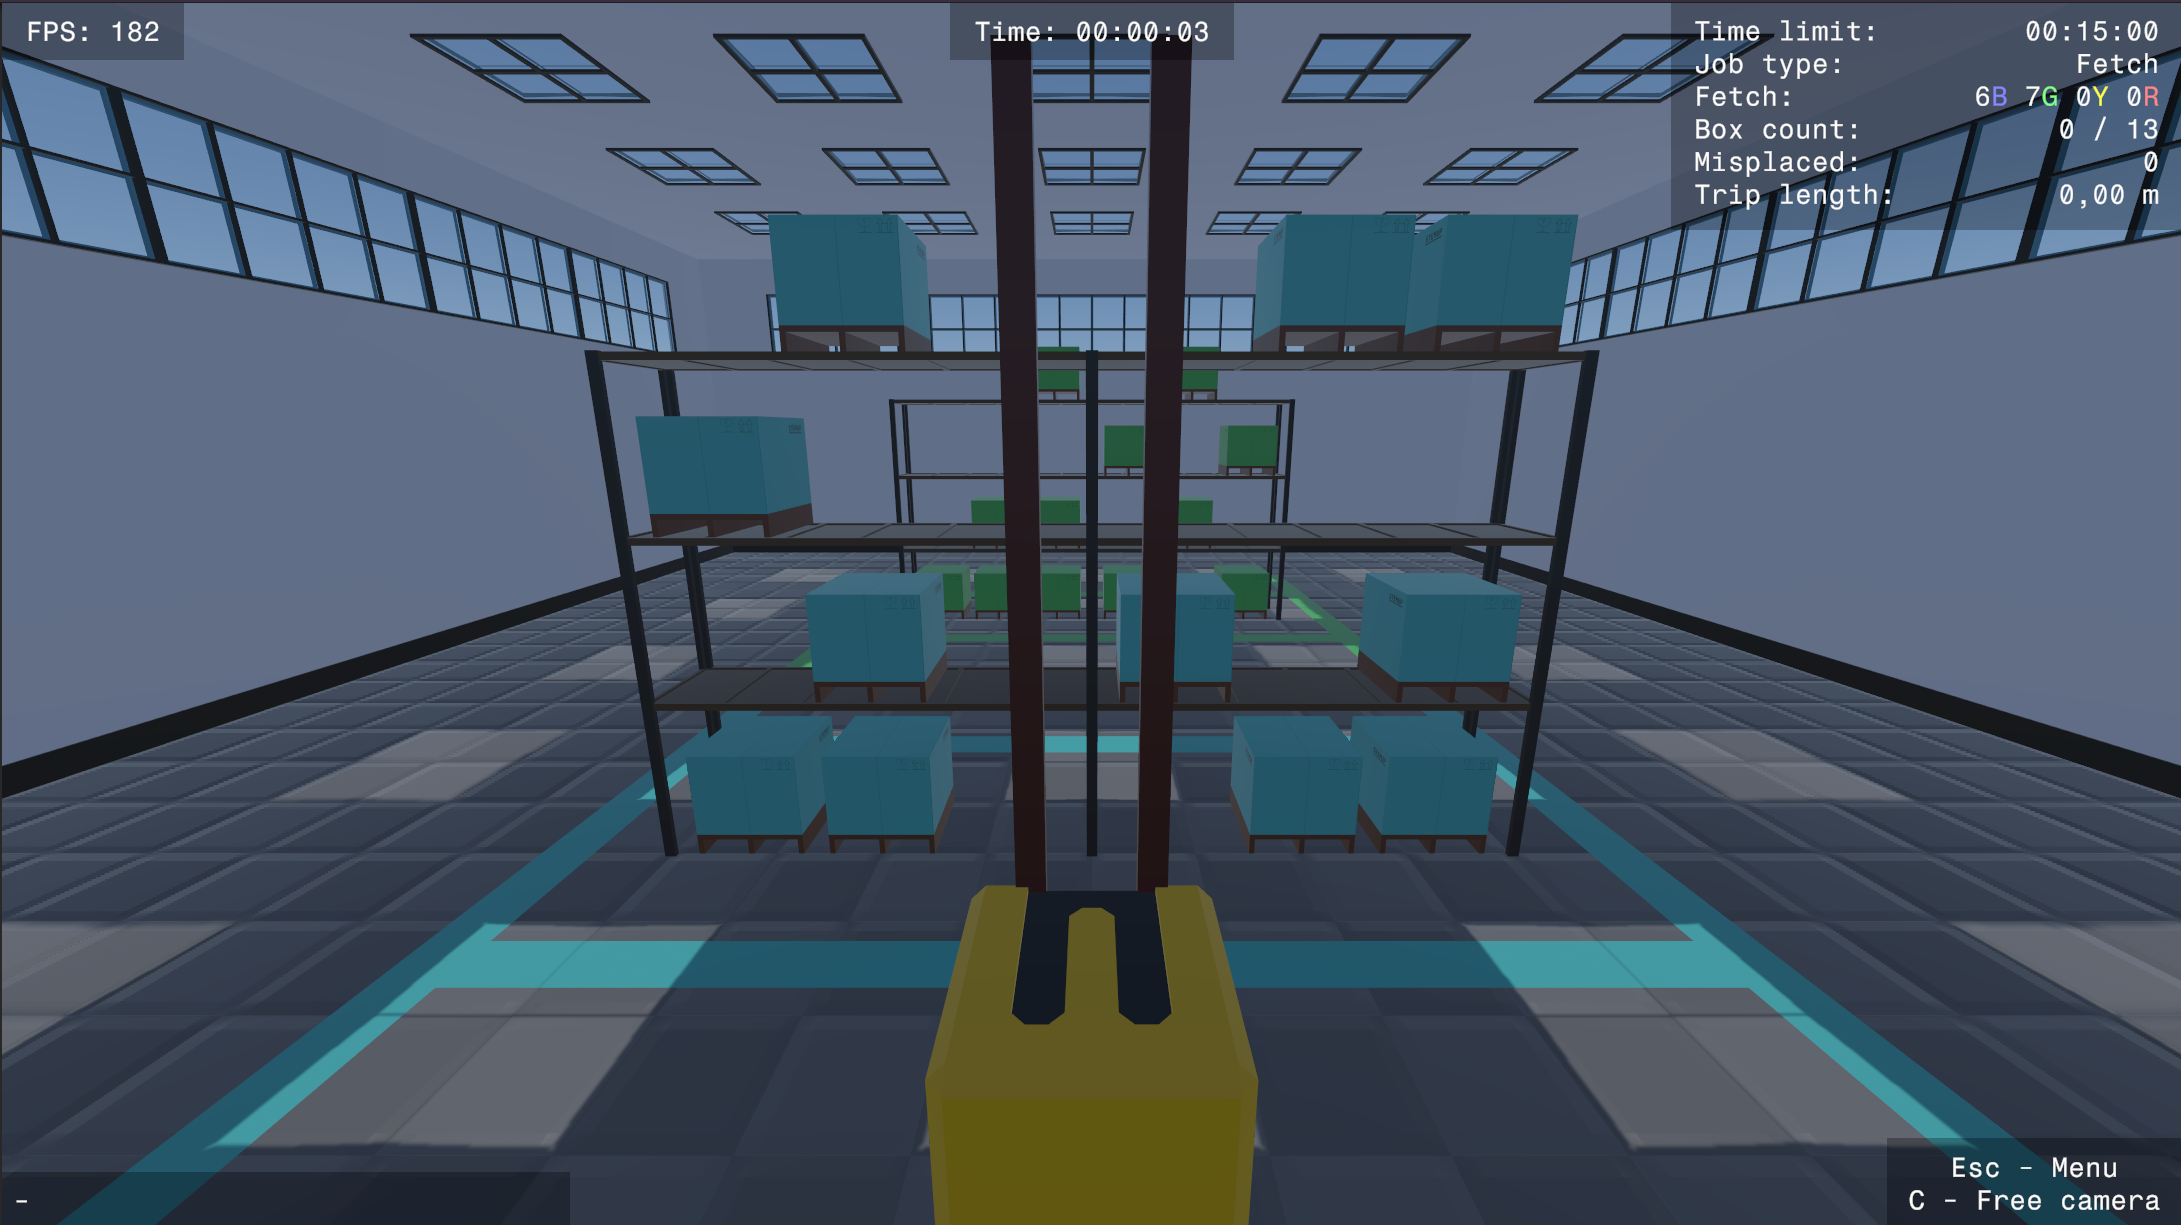
\includegraphics[width=12.1cm]{game_screen}\linebreak
    \small Screenshot of the game screen.
\end{center}

\normalsize
The game screen consists of multiple smaller elements. They're as follows:
\begin{itemize}
    \item Top left: The frames per second produced by the game, necessary to check the performance.
    \item Top middle: The timer. When it hits the time limit, the level ends.
    \item Bottom left: Additional messages are displayed here. Currently a placeholder. 
    \item Bottom right: Some of the controls are displayed here.
    \item Top right: Most of the important statistics are displayed here.
    \begin{itemize}
        \item Time limit
        \item Job type
        \item Fetch/Sort - The number of boxes that are needed to be moved.
        \item Box count - The number of boxes placed correctly out of all the necessary boxes.
        \item Misplaced - This shows the number of boxes that have been placed in an incorrect zone.
        \item Trip length - The length of the trip done by the forklift.
    \end{itemize}
\end{itemize}

\pagebreak

\section{End Screen}
\begin{center}
    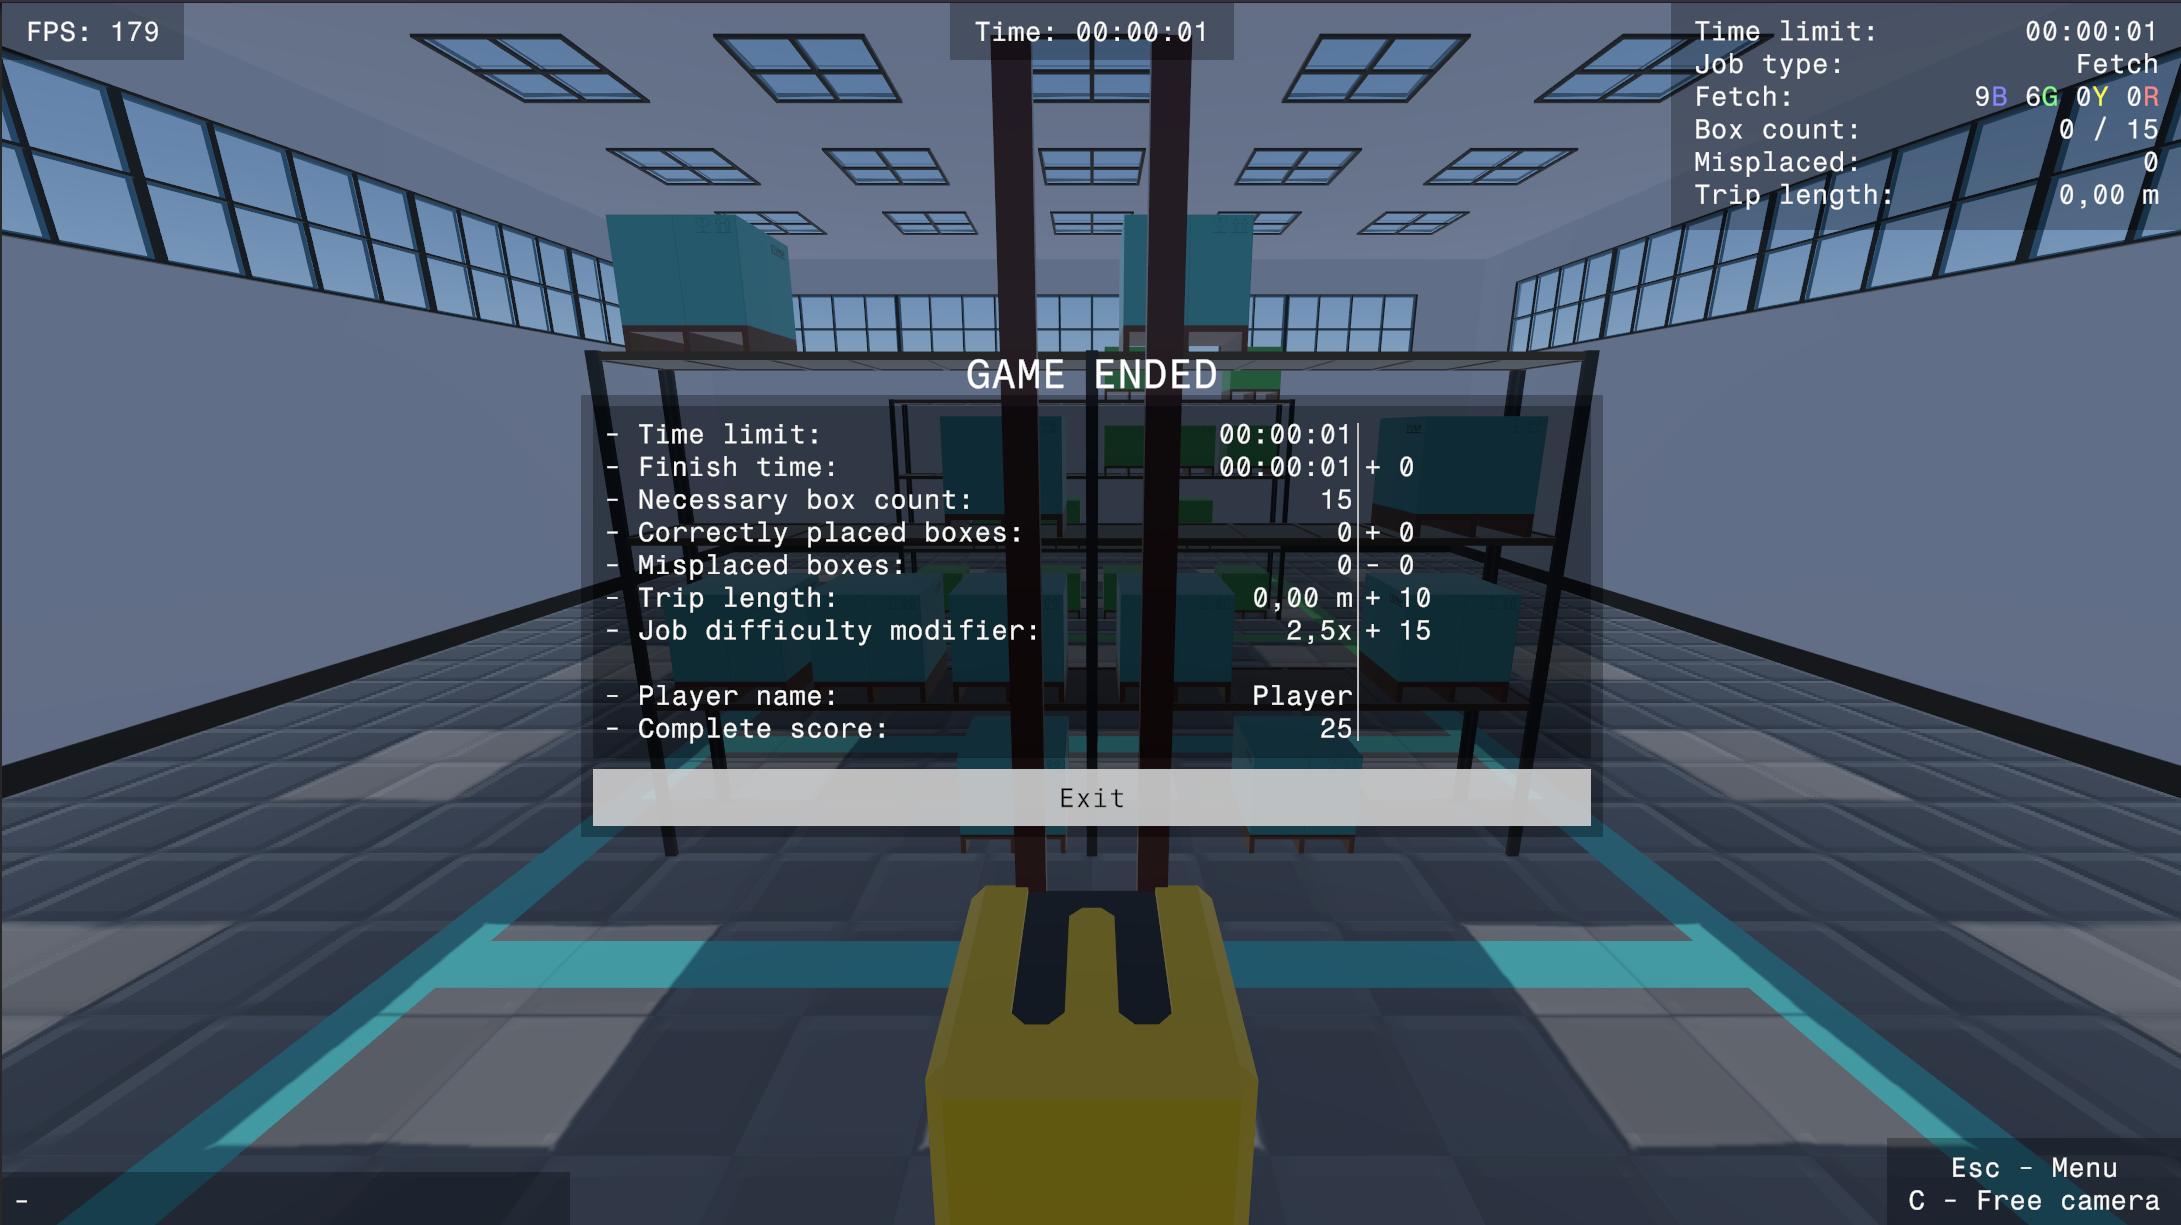
\includegraphics[width=12.1cm]{end_screen}\linebreak
    \small Screenshot of the end screen.
\end{center}

\normalsize
This screen shows the information used to calculate the score, and the final score itself.

\pagebreak

\section{Technical Documentation}
\vspace{0.25cm}
\Large \>ROS Channels \vspace{0.5cm}
\newline
\normalsize The ROS publishers:
\begin{itemize}
    \item "unityToRosTransform" - The position and rotation of the forklift within the space.
    \item "unityToRosForkHeight" - The position of the fork.
\end{itemize}
The ROS listeners:
\begin{itemize}
    \item "rosToUnityMotorSpeed" - The motor speed used while moving forwards and backward. [-1.0 / 1.0]
    \item "rosToUnityRotationSpeed" - The difference between the left and the right side used to rotate the forklift. [-1.0 / 1.0]
    \item "rosToUnityForkSpeed" - The fork's movement speed. [-1.0 / 1.0]
\end{itemize}

\end{document}